% MAT670 -- Lectures 4 and 5 (first part), transcribed from MAT670_46.pdf, pages 1--23
% Local drawing helpers for Dynkin diagrams (prefixed to avoid clashes).
% Vertices sit at (x,0); edges are drawn before vertices.
\newcommand{\LIVv}[1]{\filldraw[fill=white,draw=black] (#1) circle (0.09);}
\newcommand{\LIVe}[2]{\draw (#1) -- (#2);}
% double edge from (x,0) to (x+1,0), arrow pointing right (R) or left (L)
\newcommand{\LIVdR}[1]{\draw (#1,0.045) -- (#1+1,0.045); \draw (#1,-0.045) -- (#1+1,-0.045); \draw (#1+0.42,0.13) -- (#1+0.58,0) -- (#1+0.42,-0.13);}
\newcommand{\LIVdL}[1]{\draw (#1,0.045) -- (#1+1,0.045); \draw (#1,-0.045) -- (#1+1,-0.045); \draw (#1+0.58,0.13) -- (#1+0.42,0) -- (#1+0.58,-0.13);}
\newcommand{\LIVdN}[1]{\draw (#1,0.045) -- (#1+1,0.045); \draw (#1,-0.045) -- (#1+1,-0.045);}
% triple edge from (x,0) to (x+1,0), arrow pointing right / none
\newcommand{\LIVtR}[1]{\draw (#1,0.07) -- (#1+1,0.07); \draw (#1,0) -- (#1+1,0); \draw (#1,-0.07) -- (#1+1,-0.07); \draw (#1+0.4,0.16) -- (#1+0.6,0) -- (#1+0.4,-0.16);}
\newcommand{\LIVtN}[1]{\draw (#1,0.07) -- (#1+1,0.07); \draw (#1,0) -- (#1+1,0); \draw (#1,-0.07) -- (#1+1,-0.07);}

%======================================================================
\chapter[Lecture 4: Classification of root systems]{Lecture 4: The classification of (crystallographic) root systems}
\label{L04a:ch:L4}
\orig{Heading reads ``Lecture 4) (and 5?)''.}

%----------------------------------------------------------------------
\section{Motivation and lattice basics}
\label{L04a:sec:4.1}

In this lecture we examine \emph{root lattices}, coming from \emph{crystallographic} root systems.
One motivation is to find nice constructions of good packings in low dimensions. Another is to show
that such simple constructions do not really extend to high dimensions in a good way.
\orig{crossed out: ``there are not such simple constructions''}

The best known packings up through $\R^8$ are root lattices. In fact $A_1$, $A_2$, $A_3$ and $E_8$ are
optimal among \emph{all} packings in their dimensions.
\added{($A_1$: trivial; $A_2$: Thue, Fejes T\'oth 1940; $A_3$, the FCC packing: Hales 1998/2005, the Kepler
conjecture; $E_8$: Viazovska 2016. In dimension $24$ the Leech lattice, which is not a root lattice, is
optimal by Cohn--Kumar--Miller--Radchenko--Viazovska 2016.)}
\unclear{Box reads ``$A_1,A_2,A_3,E_8$ optimal as gen.\ packings''; ``$A_3$'' read from a blurred subscript.}

\begin{remark}
The classification we are about to give covers, in effect, half of the classification of complex
semisimple Lie algebras (equivalently, of complex semisimple Lie groups): the irreducible root systems
correspond to the simple ones.
\added{(See e.g.\ Humphreys, \emph{Introduction to Lie Algebras and Representation Theory}, Ch.~III, or
Fulton--Harris, \emph{Representation Theory}, Lecture~21.)}
\orig{Messy boxed aside, partly scribbled over; a book reference is unreadable.}
\end{remark}

\begin{definition}\label{L04a:def:lattice}
A \emph{lattice} $\Lat$ is a discrete additive subgroup of $\R^n$. For our purposes it will always be
co-compact, i.e.\ have full rank. Such a lattice has a $\Z$-basis $\{a_1,\dots,a_n\}$,
\added{$\Lat = \Z a_1\oplus\dots\oplus\Z a_n$,} that is at the same time an $\R$-basis of $\R^n$.
\end{definition}

\begin{example}
$\{(1,0)^T,(0,1)^T\}$ is a basis of the lattice $\Z^2\subset\R^2$.
\end{example}

A lattice can have many different bases. However, two bases $\{a_i\}$, $\{a_i'\}$ differ by an
\emph{integer} change of basis $K=(k_{ij})$ with integral inverse:
\[
  a_i' = \sum_{j=1}^n k_{ij} a_j, \qquad k_{ij}\in\Z
  \quad\Longrightarrow\quad \det K = \pm 1
\]
\added{(since $\det K$ and $\det K^{-1}$ are both integers whose product is $1$).}
So the volume of the torus $\R^n/\Lat$,
\[
  \vol(\R^n/\Lat) = \abs{\det\Lat} = \vol\Big(\Big\{\textstyle\sum_i t_i a_i : 0\le t_i\le 1\Big\}\Big),
\]
\added{i.e.\ the volume of the parallelepiped spanned by $a_1,\dots,a_n$, where $\det\Lat$ denotes the
determinant of the matrix with columns $a_1,\dots,a_n$,} is a clear invariant of $\Lat$.

The largest balls that can be placed at the lattice points without overlapping have radius
$\tfrac12\min_{\lambda\in\Lat\setminus\{0\}}\abs{\lambda}$, so each lattice gives a packing
\[
  \Big\{\, \varphi_i + \Ball\big(\tfrac12 \min_{\lambda\in\Lat\setminus\{0\}} \abs{\lambda}\big) \;:\; \varphi_i\in\Lat \Big\}.
\]
\begin{addedblock}
Its density is
$\dens(\Lat) = \vol \Ball^n\!\big(\tfrac12\lambda_1(\Lat)\big)\big/\abs{\det\Lat}$, where
$\lambda_1(\Lat)=\min_{\lambda\neq0}\abs{\lambda}$.
\end{addedblock}

Since scaling does not change the density, we can normalize to $\abs{\det\Lat}=1$ (i.e.\ consider
lattices $g\Z^n$ with $g\in\SL_n(\R)$).
\fixed{notes: ``(to $SL_n$, compact)''; the space is not compact}
\added{The space $\SL_n(\R)/\SL_n(\Z)$ of such lattices is \emph{not} compact (e.g.\ the lattices
$\operatorname{diag}(t,t^{-1},1,\dots,1)\Z^n$, $t\to0$, leave every compact set). What is true is
Mahler's compactness criterion: for each $\varepsilon>0$ the set of unimodular lattices with
$\lambda_1\ge\varepsilon$ is compact.}
Then there is clearly an upper bound on the length of the shortest vector among lattices with
$\abs{\det\Lat}=1$, and so a bound on the density.
\added{(Trivially, the balls are disjoint, so $\vol\Ball^n(\lambda_1/2)\le 1$; Minkowski's convex body
theorem gives the sharper $\vol\Ball^n(\lambda_1)\le 2^n$. Since lattices with very small $\lambda_1$
have small density, the supremum of the density can be taken over a set
$\{\lambda_1\ge\varepsilon\}$, which is compact by Mahler; so an optimal lattice exists in each
dimension.)}

So\dots\ what is the optimal lattice? The optimal lattice packings are known up to $n=8$
(Blichfeldt 1935 for $n=6,7,8$), and they are
\[
  A_1,\ A_2,\ A_3,\ D_4,\ D_5,\ E_6,\ E_7,\ E_8 .
\]
These are root lattices.
\orig{crossed out: ``still open''}
\added{(Earlier cases: Lagrange for $n=2$, Gauss for $n=3$, Korkine--Zolotarev for $n=4,5$. The only
other dimension where the optimal lattice is known is $n=24$: the Leech lattice, Cohn--Kumar 2009.)}

%----------------------------------------------------------------------
\section{Good candidates in low dimensions}
\label{L04a:sec:4.2}

\begin{definition}\label{L04a:def:integral}
A lattice $\Lat$ is \emph{integral} if $\ip{x}{y}\in\Z$ for all $x,y\in\Lat$.
A \emph{root lattice} is an integral lattice generated by roots, i.e.\ by elements of a root system
(Definition~\ref{L04a:def:rootsystem}).
\end{definition}

\begin{addedblock}
In lattice language one usually calls a vector $v$ of an integral lattice a root if
$\ip{v}{v}\in\{1,2\}$; then $2\ip{x}{v}/\ip{v}{v}\in\Z$ for all $x\in\Lat$, so the reflection $s_v$
(below) maps $\Lat$ to itself, and the roots of $\Lat$ form a root system. The irreducible lattices
generated by vectors of norm $2$ are exactly $A_n$ ($n\ge1$), $D_n$ ($n\ge4$), $E_6,E_7,E_8$ (Witt);
see Conway--Sloane, \emph{Sphere Packings, Lattices and Groups}, Ch.~4.
\end{addedblock}

\begin{definition}\label{L04a:def:rootsystem}
A \emph{root system} is a subset $\Delta\subset\R^n\setminus\{0\}$ satisfying:
\begin{enumerate}[label=\arabic*)]
\item $\Delta$ is finite and spans $\R^n$;
\item if $\alpha\in\Delta$, then $n\alpha\in\Delta \iff n=\pm1$ \quad(\emph{reduced});
\item $\Delta$ is invariant under the orthogonal reflection in the hyperplane $\alpha^\perp$, for any
  $\alpha\in\Delta$: writing
  \[
    \operatorname{proj}_\alpha\beta = \alpha\,\frac{\ip{\beta}{\alpha}}{\ip{\alpha}{\alpha}},\qquad
    s_\alpha\beta := \beta - 2\operatorname{proj}_\alpha\beta ,
  \]
  we require $s_\alpha\beta\in\Delta$ for all $\alpha,\beta\in\Delta$;
\item (\emph{crystallographic}) for all $\alpha,\beta\in\Delta$,
  \[
    n_{\beta\alpha} := \frac{2\ip{\beta}{\alpha}}{\ip{\alpha}{\alpha}}\in\Z .
  \]
\end{enumerate}
\added{The elements of $\Delta$ are called \emph{roots}.}
\end{definition}

\begin{center}
\begin{tikzpicture}[scale=1.1,>=Stealth]
  \draw[dashed,gray] (0,-0.4) -- (0,1.7) node[above] {\small$\alpha^\perp$};
  \draw[->,thick] (0,0) -- (2,0) node[right] {$\alpha$};
  \draw[->,thick] (0,0) -- (1.2,1.2) node[above right] {$\beta$};
  \draw[dotted] (1.2,1.2) -- (1.2,0);
  \draw[->,very thick,blue!60!black] (0,0) -- (1.2,0);
  \node[below] at (1.2,-0.05) {\small$\operatorname{proj}_\alpha\beta$};
  \draw[->,thick] (0,0) -- (-1.2,1.2) node[above left] {$s_\alpha\beta$};
  \draw[dotted] (-1.2,1.2) -- (1.2,1.2);
\end{tikzpicture}
\end{center}

Property 4) is the restriction that the projection of $\beta$ onto $\alpha$ is an integer or
half-integer multiple of $\alpha$; but it really forces $\Delta$ to give rise to a lattice
\added{(the $\Z$-span of $\Delta$ is discrete: it is the $\Z$-span of a fundamental system, which is a
basis of $\R^n$, see \S\ref{L04a:sec:4.3}).}

\begin{exercise}
Try building some other root systems, i.e.\ sets satisfying 1)--3), which are \emph{not}
crystallographic.
\added{(Hint: the $10$ unit vectors at angles $k\pi/5$ in $\R^2$; the $30$ vertices of an
icosidodecahedron in $\R^3$, i.e.\ type $H_3$.)}
\end{exercise}

\paragraph{Property 4) is strong.}
We have
\[
  n_{\beta\alpha} = \frac{2\ip{\beta}{\alpha}}{\ip{\alpha}{\alpha}} = \frac{2\abs{\beta}}{\abs{\alpha}}\cos\theta,
\]
where $\theta$ is the angle between $\alpha$ and $\beta$. Since both $n_{\beta\alpha}$ and $n_{\alpha\beta}$ are integers,
\[
  \boxed{\,n_{\beta\alpha}\,n_{\alpha\beta} = 4\cos^2\theta\in\Z\,}
  \qquad\Longrightarrow\qquad 4\cos^2\theta\in\{0,1,2,3,4\}.
\]
If $4\cos^2\theta=4$, then $\alpha$ and $\beta$ are parallel, so $\alpha=\beta$ or $\alpha=-\beta$
\added{by the reducedness axiom 2)}.

Assuming $\abs{\alpha}\ge\abs{\beta}$ (and $\alpha\neq\pm\beta$), this leaves the following table.
\begin{center}
\renewcommand{\arraystretch}{1.25}
\begin{tabular}{cccccc}
\toprule
$4\cos^2\theta$ & $n_{\beta\alpha}$ & $n_{\alpha\beta}$ & $\abs{\alpha}/\abs{\beta}$ & $\cos\theta$ & $\theta$\\
\midrule
$3$ & $+1$ & $+3$ & $\sqrt3$ & $+\sqrt3/2$ & $\pi/6$\\
$3$ & $-1$ & $-3$ & $\sqrt3$ & $-\sqrt3/2$ & $5\pi/6$\\
$2$ & $+1$ & $+2$ & $\sqrt2$ & $+\sqrt2/2$ & $\pi/4$\\
$2$ & $-1$ & $-2$ & $\sqrt2$ & $-\sqrt2/2$ & $3\pi/4$\\
$1$ & $+1$ & $+1$ & $1$ & $+1/2$ & $\pi/3$\\
$1$ & $-1$ & $-1$ & $1$ & $-1/2$ & $2\pi/3$\\
$0$ & $0$ & $0$ & (undetermined) & $0$ & $\pi/2$\\
\bottomrule
\end{tabular}
\end{center}
\added{(For $4\cos^2\theta\neq0$ the ratio follows from $n_{\alpha\beta}/n_{\beta\alpha}=\abs{\alpha}^2/\abs{\beta}^2$.)}

\begin{definition}\label{L04a:def:reducible}
A root system is \emph{reducible} (\emph{decomposable}) if $\Delta=\Delta_1\cup\Delta_2$
\added{with $\Delta_1,\Delta_2$ nonempty} such that $\ip{\alpha_1}{\alpha_2}=0$ for all
$\alpha_1\in\Delta_1$, $\alpha_2\in\Delta_2$; i.e.\ all the elements of one part are orthogonal to all
the elements of the other. Otherwise we call it \emph{irreducible} (\emph{indecomposable}).
\end{definition}

\begin{example}[Root systems in dimensions $1$ and $2$]\label{L04a:ex:rank2}
\leavevmode
\begin{center}
\begin{tikzpicture}[>=Stealth,scale=0.95]
  % A1
  \begin{scope}
    \draw[->,thick] (0,0) -- (1,0) node[right] {\small$\alpha$};
    \draw[->,thick] (0,0) -- (-1,0) node[left] {\small$-\alpha$};
    \fill (0,0) circle (1.2pt);
    \node at (0,-1.75) {$A_1$\quad($n=1$)};
  \end{scope}
  % A1 x A1
  \begin{scope}[xshift=4cm]
    \draw[->,thick] (0,0) -- (1,0) node[right] {\small$\alpha$};
    \draw[->,thick] (0,0) -- (-1,0) node[left] {\small$-\alpha$};
    \draw[->,thick] (0,0) -- (0,0.7) node[above] {\small$\beta$};
    \draw[->,thick] (0,0) -- (0,-0.7) node[below] {\small$-\beta$};
    \node at (0,-1.75) {$A_1\times A_1$\ (reducible), $\theta=\frac\pi2$};
  \end{scope}
  % A2
  \begin{scope}[xshift=9.4cm]
    \draw[gray!60] (0:1)--(60:1)--(120:1)--(180:1)--(240:1)--(300:1)--cycle;
    \foreach \a in {0,60,...,300} \draw[->,thick] (0,0) -- (\a:1);
    \node[right] at (0:1) {\small$\alpha$};
    \node[above left] at (120:1) {\small$\beta$};
    \node[above right] at (60:1) {\small$\alpha+\beta=s_\alpha\beta$};
    \node[left] at (180:1) {\small$-\alpha$};
    \node[below left] at (240:1) {\small$s_\alpha(-\beta)$};
    \node[below right] at (300:1) {\small$-\beta$};
    \node at (0,-1.75) {$A_2$, $\theta=\frac\pi3$};
  \end{scope}
\end{tikzpicture}

\medskip
\begin{tikzpicture}[>=Stealth,scale=0.95]
  % B2
  \begin{scope}
    \draw[gray!60] (-1,-1) rectangle (1,1);
    \foreach \v in {(1,0),(0,1),(-1,0),(0,-1),(1,1),(-1,1),(-1,-1),(1,-1)} \draw[->,thick] (0,0) -- \v;
    \node[right] at (1,0) {\small$\alpha$};
    \node[above left] at (-1,1) {\small$\beta$};
    \node[above] at (0,1) {\small$s_\beta\alpha$};
    \node at (0,-1.5) {$B_2$, $\theta=\frac\pi4$};
  \end{scope}
  % G2
  \begin{scope}[xshift=5cm]
    \foreach \a in {0,60,...,300} \draw[->,thick] (0,0) -- (\a:0.7);
    \foreach \a in {30,90,...,330} \draw[->,thick] (0,0) -- (\a:1.212);
    \draw[gray!60] (30:1.212)--(150:1.212)--(270:1.212)--cycle;
    \draw[gray!60] (90:1.212)--(210:1.212)--(330:1.212)--cycle;
    \node at (0,-1.5) {$G_2$, $\theta=\frac\pi6$};
  \end{scope}
\end{tikzpicture}
\end{center}
(Note: $\Delta$ is not a basis!)
\added{In $B_2$ the roots are $\pm e_1,\pm e_2,\pm e_1\pm e_2$; in $G_2$ there are $6$ short roots and
$6$ long roots of length ratio $\sqrt3$. In each case $\theta$ is the smallest angle between two roots.}
\end{example}

%----------------------------------------------------------------------
\section{Classification of root systems: preliminaries}
\label{L04a:sec:4.3}

From a root system $\Delta$ we can choose a (non-unique) subset, the \emph{simple roots}.

For each $\alpha\in\Delta$ consider $\alpha^\perp$, its (linear) orthogonal complement.
\orig{crossed out: ``there is a unique $\perp$ hyperplane''}
Since $\abs{\Delta}$ is finite, there exists $d\in\R^n$ such that $\ip{\alpha}{d}\neq0$ for all
$\alpha\in\Delta$ \added{(avoid the finitely many hyperplanes $\alpha^\perp$)}. Hence there is a
partition of $\Delta$ into
\[
  \text{positive roots } \Delta_d^+ = \{\alpha\in\Delta : \ip{\alpha}{d}>0\},\qquad
  \text{negative roots } \Delta_d^- = \{\alpha\in\Delta : \ip{\alpha}{d}<0\}
\]
\added{(note $\Delta_d^-=-\Delta_d^+$).}

\begin{definition}\label{L04a:def:simple}
A root $\alpha\in\Delta_d^+$ is \emph{simple} if it is not the sum of two other positive roots.
A set of simple roots is a \emph{fundamental system} of $\Delta$ \added{(we write $\Pi=\Pi_d$)}.
\end{definition}

\begin{center}
\begin{tikzpicture}[>=Stealth,scale=1.3]
  \fill[gray!12] (165:1.7) -- (-15:1.7) arc (-15:165:1.7) -- cycle;
  \draw[dashed,red!70!black] (165:1.8) -- (-15:1.8) node[right] {\small$d^\perp$};
  \foreach \a in {0,60,...,300} \draw[->,thick] (0,0) -- (\a:1.2);
  \node[right] at (0:1.2) {\small$\alpha$};
  \node[above left] at (120:1.2) {\small$\beta$};
  \node[above right] at (60:1.2) {\small$\alpha+\beta$};
  \draw[->,red!70!black,thick] (0,0) -- (75:0.9) node[above] {\small$d$};
  \node at (35:1.75) {\small$\Delta_d^+$};
  \node at (-110:1.4) {\small$\Delta_d^-$};
\end{tikzpicture}
\end{center}
\orig{Sketch on p.\,8, redrawn for $A_2$: simple roots $\alpha,\beta$.}

The choice of $d$ affects the fundamental system, but such systems are equivalent under the action of
the group of reflections $\langle s_\alpha\rangle_{\alpha\in\Delta}$
\added{(the \emph{Weyl group} $W$; see Proposition~\ref{L04a:prop:reconstruct}).}

\begin{theorem}\label{L04a:thm:basis}
A fundamental system of $\Delta$ is an $\R$-basis for $\R^n$.
\added{Moreover every positive root is a linear combination of simple roots with nonnegative integer
coefficients.}
\end{theorem}

\begin{proof}[Sketch]
\emph{Linear independence.} Suppose $\sum_i c_i\gamma_i = 0$ with $\gamma_i\in\Pi$. Partition the
indices into those with $c_i>0$ $(+)$, those with $c_i<0$ $(-)$, and those with $c_i=0$, and put
\added{$x := \sum_{c_i>0} c_i\gamma_i = \sum_{c_j<0}\abs{c_j}\gamma_j$.} Then
\[
  \ip{x}{x} = \sum_{c_i>0,\ c_j<0} c_i\,\abs{c_j}\,\ip{\gamma_i}{\gamma_j}\le 0
\]
by Lemma~\ref{L04a:lem:obtuse} (distinct simple roots make non-acute angles), so $x=0$.
\added{But then $0=\ip{x}{d}=\sum_{c_i>0}c_i\ip{\gamma_i}{d}$ with every $\ip{\gamma_i}{d}>0$, so no
$c_i$ is positive; likewise none is negative.}

\emph{Span.} Let $\gamma$ be orthogonal to all simple roots. Then by the orbit argument
(Proposition~\ref{L04a:prop:reconstruct}: every root is the image of a simple root under the group
generated by the simple reflections $s_\alpha$, $\alpha\in\Pi$, each of which fixes $\gamma$),
$\gamma$ is orthogonal to all roots, hence $\gamma=0$ since $\Delta$ spans.
\begin{addedblock}
A more elementary route: if $\alpha\in\Delta_d^+$ is not simple, then $\alpha=\beta+\beta'$ with
$\beta,\beta'\in\Delta_d^+$, and $\ip{\beta}{d},\ip{\beta'}{d}<\ip{\alpha}{d}$. Since $\Delta$ is
finite, induction on $\ip{\alpha}{d}$ shows every positive root is a sum of simple roots. Hence $\Pi$
spans $\operatorname{span}\Delta=\R^n$, and the integrality claim follows too.
\end{addedblock}
\end{proof}

\begin{proposition}\label{L04a:prop:reconstruct}
$\Delta$ can be reconstructed from a fundamental system via reflections.
\added{Precisely: if $W_\Pi$ denotes the group generated by $s_\gamma$, $\gamma\in\Pi$, then
$\Delta = W_\Pi\cdot\Pi$, and any two fundamental systems are related by an element of $W_\Pi$.}
\end{proposition}

\begin{proof}[Sketch]
Consider the \emph{Weyl chamber} of the fundamental system $\Pi$,
\[
  C(\Pi)=\{x\in\R^n : \ip{x}{\gamma}>0 \text{ for all }\gamma\in\Pi\}.
\]
\orig{crossed out: ``orbit $d$ to each\dots''}
Then $d\in C(\Pi)$, and moving $d$ within its chamber does not change the fundamental system.
Any other fundamental system is based on some $d'$ in another chamber, and there are finitely many
chambers \added{(the connected components of $\R^n\setminus\bigcup_{\alpha}\alpha^\perp$)}. Take a path
$d\to d'$ \added{in general position}; the walls it crosses give reflections $s_{\text{walls}}$, whose
composition takes $d$ to (the chamber of) $d'$, and hence takes the fundamental system of $d$ to that
of $d'$.
\begin{addedblock}
Details: if $d$ and $d'=s_\alpha d$ lie in adjacent chambers separated by the wall $\alpha^\perp$,
then $\Pi_{d'}=s_\alpha\Pi_d$, since $s_\alpha$ is an isometry permuting $\Delta$ with
$\ip{s_\alpha\beta}{s_\alpha d}=\ip{\beta}{d}$. The walls of $C(\Pi)$ are exactly the hyperplanes
$\gamma^\perp$, $\gamma\in\Pi$; writing each wall-crossing reflection in terms of the previous ones
($s_{w\gamma}=ws_\gamma w^{-1}$) shows the composite lies in $W_\Pi$. Finally every root $\alpha$ is
simple for a suitable $d'$ (take $d'$ very close to a generic point of $\alpha^\perp$, on the side where
$\ip{\alpha}{d'}>0$), so $\alpha=w\gamma$ for some $w\in W_\Pi$, $\gamma\in\Pi$. See Humphreys,
\emph{Introduction to Lie Algebras and Representation Theory}, \S10.3.
\end{addedblock}
\end{proof}

\begin{center}
\begin{tikzpicture}[>=Stealth,scale=1.6]
  % hyperplanes alpha^perp (90), beta^perp (30), (alpha+beta)^perp (150)
  \draw[magenta,thick] (90:1.5) -- (270:1.5) node[below] {\small$\alpha^\perp$};
  \draw[magenta,thick] (30:1.5) -- (210:1.5) node[below left] {\small$\beta^\perp$};
  \draw[magenta,thick] (150:1.5) -- (330:1.5) node[below right] {\small$(\alpha+\beta)^\perp$};
  \foreach \a in {0,60,...,300} \draw[->,thick] (0,0) -- (\a:1.15);
  \node[right] at (0:1.15) {\small$\alpha$};
  \node[left] at (180:1.15) {\small$s_\alpha(\alpha)$};
  \node[above left] at (120:1.15) {\small$\beta=s_\alpha(\alpha+\beta)$};
  \node[above right] at (60:1.15) {\small$\alpha+\beta=s_\alpha(\beta)$};
  \fill[red!70!black] (75:0.8) circle (1pt) node[right] {\small$d$};
  \fill[green!45!black] (105:0.8) circle (1pt) node[left] {\small$s_\alpha d$};
  \draw[dashed] (75:0.8) to[bend right=15] (105:0.8);
\end{tikzpicture}
\end{center}
\orig{Colour sketch on p.\,11, redrawn.}
For $A_2$: with $d$ as shown, $\Pi_d=\{\alpha,\beta\}$; reflecting across $\alpha^\perp$ gives
$s_\alpha d$, with fundamental system $\Pi_{s_\alpha d}=\{s_\alpha(\alpha),s_\alpha(\beta)\}=\{-\alpha,\alpha+\beta\}$.

\begin{lemma}\label{L04a:lem:diff}
If $\alpha,\beta\in\Delta$ are not parallel and $\ip{\alpha}{\beta}>0$, then $\alpha-\beta\in\Delta$.
\end{lemma}

\begin{proof}
We have $n_{\alpha\beta}=2\ip{\alpha}{\beta}/\ip{\beta}{\beta}>0$, and by the table
\added{($n_{\alpha\beta}n_{\beta\alpha}\in\{1,2,3\}$ with both factors positive integers)}
$n_{\alpha\beta}=1$ or $n_{\beta\alpha}=1$. If $n_{\alpha\beta}=1$, then
\[
  s_\beta(\alpha) = \alpha - 2\beta\,\frac{\ip{\alpha}{\beta}}{\ip{\beta}{\beta}}
  = \alpha-n_{\alpha\beta}\,\beta = \alpha-\beta\in\Delta.
\]
Similarly, if $n_{\beta\alpha}=1$, then $s_\alpha(-\beta)=-\beta+n_{\beta\alpha}\alpha=\alpha-\beta\in\Delta$.
\fixed{written $m_{\beta\alpha}$, $s_\beta(-\beta)$ (typos)}
\end{proof}

\begin{lemma}\label{L04a:lem:obtuse}
If $\alpha,\beta$ are distinct simple roots, then $\ip{\alpha}{\beta}\le0$.
\end{lemma}

\begin{proof}
If $\ip{\alpha}{\beta}>0$, then \added{(as $\alpha\neq\pm\beta$, both being positive)}
Lemma~\ref{L04a:lem:diff} gives $\gamma:=\alpha-\beta\in\Delta$. So $\gamma$ or $-\gamma$ lies in
$\Delta_d^+$, and then $\alpha=\beta+\gamma$ or $\beta=\alpha+(-\gamma)$ is a sum of two positive roots,
contradicting simplicity.
\end{proof}

\begin{proposition}\label{L04a:prop:decomp}
A fundamental system is decomposable \added{(into two nonempty mutually orthogonal subsets)} if and only
if the root system is decomposable.
\end{proposition}

\begin{proof}[Sketch]
Similar arguments.
\begin{addedblock}
If $\Delta=\Delta_1\cup\Delta_2$ orthogonally, then $\Pi=(\Pi\cap\Delta_1)\cup(\Pi\cap\Delta_2)$, and
both parts are nonempty because $\Pi$ spans $\R^n$. Conversely, if $\Pi=\Pi_1\cup\Pi_2$ orthogonally,
the reflections $s_\gamma$, $\gamma\in\Pi_1$, fix $\Pi_2$ pointwise and preserve
$\operatorname{span}\Pi_1$, and vice versa; so by
Proposition~\ref{L04a:prop:reconstruct} every root lies in $W_\Pi\Pi_1\subset\operatorname{span}\Pi_1$ or
in $W_\Pi\Pi_2\subset\operatorname{span}\Pi_2$, which are orthogonal.
\end{addedblock}
\end{proof}

%----------------------------------------------------------------------
\section{Classification via Coxeter graphs}
\label{L04a:sec:4.4}

Simple roots determine root systems (Proposition~\ref{L04a:prop:reconstruct}), so it is enough to
classify fundamental systems.

Elements $\alpha,\beta$ of a fundamental system are orthogonal or make an obtuse angle
(Lemma~\ref{L04a:lem:obtuse}). By the table, therefore,
\[
  \theta \in \Big\{\frac\pi2,\ \frac{2\pi}3,\ \frac{3\pi}4,\ \frac{5\pi}6\Big\},
  \qquad\text{that is,}\qquad n_{\alpha\beta}n_{\beta\alpha}=4\cos^2\theta\in\{0,1,2,3\}.
\]

\begin{definition}\label{L04a:def:coxeter}
The \emph{Coxeter graph} of $\Delta$ has a vertex for each simple root, and an edge of weight
$n_{\alpha\beta}\cdot n_{\beta\alpha}$ between $\alpha$ and $\beta$ \added{(drawn as that many edges;
no edge when $\alpha\perp\beta$)}.
\end{definition}

It is well defined \added{(independent of the choice of fundamental system)} by the Weyl chamber
argument, since fundamental systems are carried to fundamental systems by the reflections
$\langle s_\alpha\rangle$, \added{which are isometries and so preserve all the angles}.

\begin{definition}\label{L04a:def:dynkin}
The \emph{Dynkin diagram} is the Coxeter graph with arrows on the double and triple edges, pointing to
the shorter vector.
\end{definition}

\begin{remark}
In an irreducible system, the possible lengths are determined by the angles
\added{(by the table, the ratio of the lengths of two non-orthogonal roots is fixed by their angle;
connecting through the diagram fixes all lengths up to one overall scale)}. For a reducible system the
components can be rescaled independently.
\unclear{Margin note by $A_1\times A_1$, probably ``unrelated scale!''.}
\end{remark}

\begin{example}
\leavevmode
\begin{center}
\begin{tabular}{r@{\quad$\longrightarrow$\quad}l}
$A_1$ & \tikz[baseline=-3pt]{\LIVv{0,0}} \\[4pt]
$A_1\times A_1$ & \tikz[baseline=-3pt]{\LIVv{0,0}\LIVv{1,0}} \\[4pt]
$A_2$ & \tikz[baseline=-3pt]{\LIVe{0,0}{1,0}\LIVv{0,0}\LIVv{1,0}} \\[4pt]
$B_2$ & \tikz[baseline=-3pt]{\LIVdR{0}\LIVv{0,0}\LIVv{1,0}} \\[4pt]
$G_2$ & \tikz[baseline=-3pt]{\LIVtR{0}\LIVv{0,0}\LIVv{1,0}}
\end{tabular}
\end{center}
\end{example}

\orig{End of Lecture 4 (p.\,15).}

%======================================================================
\chapter[Lecture 5: Root systems (continued)]{Lecture 5: Classification of crystallographic root systems (continued)}
\label{L04a:ch:L5}

\paragraph{Recall.} A root system $\Delta\subset\R^n\setminus\{0\}$ satisfies
\begin{enumerate}[label=\arabic*)]
\item $\Delta$ is finite and spans $\R^n$;
\item $\alpha\in\Delta\implies(n\alpha\in\Delta\iff n=\pm1)$;
\item $\Delta$ is invariant under the reflections in the hyperplanes $\alpha^\perp$:
  $s_\alpha(\beta)\in\Delta$ for all $\alpha,\beta\in\Delta$;
\item $n_{\beta\alpha}:=2\ip{\beta}{\alpha}/\ip{\alpha}{\alpha}\in\Z$,
\end{enumerate}
and 4) implies $4\cos^2\theta_{\alpha\beta}\in\Z$, really $\in\{0,1,2,3,4\}$.

The plan: root lattices $\to$ root systems $\longleftrightarrow$ simple roots (last time)
$\longleftrightarrow$ Dynkin diagrams (today).

From \S\ref{L04a:sec:4.4}: the \emph{Coxeter graph} has a vertex for each simple root and an edge of
weight $n_{\alpha\beta}\cdot n_{\beta\alpha}$ between $\alpha$ and $\beta$. The \emph{Dynkin diagram} is
the Coxeter graph with arrows on the multi-edges pointing at the shorter root.
\orig{Page has ``(longer)'' with ``shorter'' written below.}

%----------------------------------------------------------------------
\section{Classification of Coxeter graphs}
\label{L04a:sec:5.1}

We ignore lengths.

\begin{definition}\label{L04a:def:admissible}
A linearly independent set of $n$ unit vectors $\{v_1,\dots,v_n\}$ spanning $\R^n$ is \emph{admissible}
if for all $i\neq j$
\[
  \ip{v_i}{v_j}\le0 \qquad\text{and}\qquad 4\ip{v_i}{v_j}^2 = 4\cos^2\theta_{ij}\in\{0,1,2,3\}.
\]
An \emph{admissible diagram} is the Coxeter graph of an admissible set
\added{(vertices $v_i$, with $4\ip{v_i}{v_j}^2$ edges between $v_i$ and $v_j$)}.
\end{definition}

\begin{center}
\fbox{\parbox{0.8\linewidth}{\centering A normalized set of simple roots is admissible.\\
(Note: the angles are the determining factor.)}}
\end{center}
\added{This follows from Theorem~\ref{L04a:thm:basis}, Lemma~\ref{L04a:lem:obtuse} and the table.}

The simple roots of an irreducible $\Delta$ are not all orthogonal
\added{--- more precisely, they cannot be split into two mutually orthogonal sets
(Proposition~\ref{L04a:prop:decomp})} --- so the Coxeter graph is connected. So we only need to classify
connected admissible diagrams.

\begin{theorem}\label{L04a:thm:classification}
The Dynkin diagram of an irreducible (crystallographic) root system is of one of the following types
($n$ = number of vertices).

\smallskip
\noindent\emph{Infinite families:}
\begin{center}
\begin{tabular}{lll}
$A_n$ & \tikz[baseline=-3pt]{\LIVe{0,0}{1,0}\draw[dotted] (1,0)--(2,0);\LIVe{2,0}{3,0}\foreach\x in{0,1,2,3}{\LIVv{\x,0}}} & $n\ge1$\\[6pt]
$B_n$ & \tikz[baseline=-3pt]{\LIVe{0,0}{1,0}\draw[dotted] (1,0)--(2,0);\LIVdR{2}\foreach\x in{0,1,2,3}{\LIVv{\x,0}}} & $n\ge2$\\[6pt]
$C_n$ & \tikz[baseline=-3pt]{\LIVe{0,0}{1,0}\draw[dotted] (1,0)--(2,0);\LIVdL{2}\foreach\x in{0,1,2,3}{\LIVv{\x,0}}} & $n\ge3$\\[6pt]
$D_n$ & \tikz[baseline=-3pt]{\LIVe{0,0}{1,0}\draw[dotted] (1,0)--(2,0);\LIVe{2,0}{2.8,0.45}\LIVe{2,0}{2.8,-0.45}\foreach\x in{0,1,2}{\LIVv{\x,0}}\LIVv{2.8,0.45}\LIVv{2.8,-0.45}} & $n\ge4$
\end{tabular}
\end{center}

\noindent\emph{Exceptional types:}
\begin{center}
\begin{tabular}{ll}
$E_6$ & \tikz[baseline=-3pt]{\foreach\x in{0,1,2,3}{\LIVe{\x,0}{\x+1,0}}\LIVe{2,0}{2,0.7}\foreach\x in{0,...,4}{\LIVv{\x,0}}\LIVv{2,0.7}}\\[12pt]
$E_7$ & \tikz[baseline=-3pt]{\foreach\x in{0,...,4}{\LIVe{\x,0}{\x+1,0}}\LIVe{2,0}{2,0.7}\foreach\x in{0,...,5}{\LIVv{\x,0}}\LIVv{2,0.7}}\\[12pt]
$E_8$ & \tikz[baseline=-3pt]{\foreach\x in{0,...,5}{\LIVe{\x,0}{\x+1,0}}\LIVe{2,0}{2,0.7}\foreach\x in{0,...,6}{\LIVv{\x,0}}\LIVv{2,0.7}}\\[6pt]
$F_4$ & \tikz[baseline=-3pt]{\LIVe{0,0}{1,0}\LIVdR{1}\LIVe{2,0}{3,0}\foreach\x in{0,...,3}{\LIVv{\x,0}}}\\[6pt]
$G_2$ & \tikz[baseline=-3pt]{\LIVtR{0}\LIVv{0,0}\LIVv{1,0}}
\end{tabular}
\end{center}
\added{Conversely, each of these diagrams is the Dynkin diagram of an irreducible root system, which is
unique up to isomorphism.}
\unclear{Parenthetical under $D_n$ reads roughly ``(each also unique)''.}
\added{(The ranges of $n$ avoid repetitions: $B_2=C_2$, $D_3=A_3$.)}
\end{theorem}

It will suffice to classify admissible diagrams. By definition, subsets of the vectors of an admissible
set satisfy the admissibility condition inside their span (the resulting diagram could be
disconnected); \added{that is, any subdiagram of an admissible diagram, obtained by deleting vertices,
is admissible.}

\begin{lemma}\label{L04a:lem:tree}
A connected admissible diagram is a tree.
\end{lemma}

\begin{proof}
Consider $v=\sum_{i=1}^n v_i$, where $\{v_i\}$ is admissible. The $v_i$ are linearly independent, so
$v\neq0$, and
\[
  0<\ip{v}{v} = \sum_i\ip{v_i}{v_i} + \sum_{i<j}2\ip{v_i}{v_j} = n+\sum_{i<j}2\ip{v_i}{v_j}.
\]
If $v_i$ is connected to $v_j$ in the Coxeter graph, then by the table
$2\ip{v_i}{v_j}\in\{-1,-\sqrt2,-\sqrt3\}$\added{, in particular $2\ip{v_i}{v_j}\le-1$}. Hence
$\sum_{i<j}2\ip{v_i}{v_j}$ has at most $n-1$ terms not equal to $0$, i.e.\ there are at most $n-1$
connected pairs of vertices. But by assumption the diagram is connected, so there are exactly $n-1$
pairs of connected vertices \added{(a connected graph on $n$ vertices has at least $n-1$ edges)}, and
it is a tree (maybe with multiple edges, but not too many).
\orig{a scribbled-out remark at the bottom of p.\,20}
\end{proof}

\begin{lemma}\label{L04a:lem:degree}
The degree of each vertex, counted with multiplicity, is at most $3$.
\end{lemma}

\begin{proof}
Fix a vertex $v$, connected to the vertices $v_1,\dots,v_k$.
\fixed{written ``fix vertex $v_1$'', then used as $v$}
Since the diagram is a tree \added{(Lemma~\ref{L04a:lem:tree}, applied to the subdiagram on
$v,v_1,\dots,v_k$)}, $\ip{v_i}{v_j}=0$ for $i\neq j$, so $\{v_1,\dots,v_k\}$ is orthonormal. Also,
$\{v_1,\dots,v_k,v\}$ is linearly independent (by admissibility; for simple roots this is Theorem~\ref{L04a:thm:basis}), so
the normalized projection
\[
  v_0 := \frac{\operatorname{proj}_{\langle v_1,\dots,v_k\rangle^\perp}(v)}{\norm{\operatorname{proj}_{\langle v_1,\dots,v_k\rangle^\perp}(v)}}
\]
is defined, and $\ip{v}{v_0}\neq0$. Now $\{v_0,\dots,v_k\}$ is an orthonormal set, and $v$ lies in its
span, so
\[
  v=\sum_{i=0}^k\ip{v}{v_i}v_i \qquad\text{and}\qquad \ip{v}{v}=\sum_{i=0}^k\ip{v}{v_i}^2=1 .
\]
Since $\ip{v}{v_0}^2\neq0$,
\[
  \sum_{i=1}^k 4\ip{v}{v_i}^2<4 .
\]
But $4\cos^2\theta = 4\ip{v}{v_i}^2$ is the number of edges from $v$ to $v_i$. So the degree of $v$,
counted with multiplicity, is at most $3$.
\end{proof}

\begin{corollary}\label{L04a:cor:G2}
\tikz[baseline=-3pt]{\LIVtN{0}\LIVv{0,0}\LIVv{1,0}} is the only connected admissible diagram with a
triple edge.
\end{corollary}

\begin{proof}[\added{Proof}]
\added{If $v$ and $w$ are joined by a triple edge, both already have degree $3$, so by
Lemma~\ref{L04a:lem:degree} neither is joined to any other vertex; by connectedness there are no
other vertices.}
\end{proof}

So from now on we consider only double and single edges.

\begin{definition}\label{L04a:def:chain}
A \emph{simple chain} is a collection of vertices connected by single edges:
\begin{center}
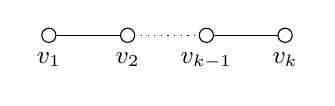
\begin{tikzpicture}
  \LIVe{0,0}{1,0}\draw[dotted] (1,0)--(2,0);\LIVe{2,0}{3,0}
  \foreach\x in{0,1,2,3}{\LIVv{\x,0}}
  \node[below] at (0,-0.1) {\small$v_1$};
  \node[below] at (1,-0.1) {\small$v_2$};
  \node[below] at (2,-0.1) {\small$v_{k-1}$};
  \node[below] at (3,-0.1) {\small$v_k$};
\end{tikzpicture}
\end{center}
\end{definition}

\begin{lemma}[Simple chain collapse]\label{L04a:lem:collapse}
In an admissible diagram, a simple chain represented by $\{v_1,\dots,v_k\}$ can be replaced by the single
vector $v=\sum_{i=1}^k v_i$, giving an admissible diagram.
\end{lemma}

\begin{proof}
We want to show that $v$ is a unit vector and that the collapsed diagram is admissible.
\added{(Linear independence of the new set is clear, since the $v_i$ and the remaining vectors are
linearly independent.)}
We have
\[
  \ip{v}{v} = k + \sum_{i<j}2\ip{v_i}{v_j},
\]
and $\ip{v_i}{v_j}=0$ for all $i<j$ except $j=i+1$ \added{(a tree has no other edges among the $v_i$)}.
For a single edge, recall $2\ip{v_i}{v_{i+1}}=-1$. Hence
\[
  \ip{v}{v} = k-(k-1) = 1 .
\]
Now consider a vertex $u$ not represented in the chain. It connects to at most one vertex in the chain
(by the tree property), say $v_j$ \added{(if none, $\ip{u}{v}=0$)}. Then
\[
  \ip{u}{v}=\sum_{i=1}^k\ip{u}{v_i}=\ip{u}{v_j},
\]
so the angles $\theta_{u,v}$ and $\theta_{u,v_j}$ are the same, and the collapsed set is admissible.
\orig{scribbled-out ``recall admissible\dots'' at the foot of p.\,23}
\end{proof}
